\documentclass[../../../main.tex]{subfiles}

\begin{document}

The method described here to represent spins in terms of Fermions was first employed by Abrikosov in 1965 and later reformulated in terms of gauge theory by Affleck in 1988. The idea (for spin 1/2!) is to introduce two new flavours of fermions: $c_{i\uparrow}^\dagger, \, c_{i\downarrow}^\dagger$ on each site. The transformation reads

\begin{equation}\label{Abrfer}
\vec{S}_i = \frac12 \sum_{\alpha, \beta} c_{i\alpha}^\dagger \vec{\sigma}_{\alpha \beta} c_{i\beta},
\end{equation}

where $\vec{\sigma}$ is the vector of Pauli matrices. \\

This transformation is quite natural, as it has been found even before Abrikosov, just the other way around. It is known that the large-U limit of the Hubbard model at half-filling gives a antiferromagnetic Heisenberg model. In the perturbation theory one finds the exact representation of Spins in terms of fermionic ladder operators given above.

\subsubsection{Hilbert space and un-physical states}

The mapping \ref{Abrfer} is exact on the operator level, meaning, that the eigenspaces of $S_i^2$ and $S_i^\alpha$ remain unchanged. \\ 

The local Hilbert space, however, gets enlarged. We drop the site-indices from now on. The spin-1/2 Hilbert space is of course a two-dimensional Hilbert space

\begin{equation}
\mathcal{H}_{S=\frac12} =  \text{span}\left(\ket{\uparrow}, \ket{\downarrow} \right)
\end{equation}

The two-fermion Hilbert space on the other hand is four-dimenstional

\begin{equation}
	\mathcal{H}_{\text{fermions}} = \text{span}\left(\ket{00}, \ket{10}, \ket{01}, \ket{11}\right).
\end{equation}

The idea of \ref{Abrfer} is to identify $\mathcal{H}_{S=\frac12}$ with the one-particle sector of $\mathcal{H}_{\text{fermions}}$:

\begin{equation}\label{strong_constr}
	\left(n_{i\uparrow} + n_{i\downarrow}\right)\ket{\psi} \overset{!}{=} \ket{\psi} \; \forall i.
\end{equation}

This leaves us with two un-physical states: $\ket{00}$ and $\ket{11}$. \\


All spin-operators $S^\alpha$ act trivially on these, which is why everything goes through smoothly on the operator level. Therefore, as long as the Hamiltonian only consists of spin operators, the un-physical states do not influence any results (apart from normalization, maybe). \\

This can not be garuanteed anymore when treating the system perturbatively using for example a mean-field theory. For this reason we introduce the constraint 

\begin{equation}\label{weak_constr}
\bra{\psi} n_{i\downarrow} + n_{i\uparrow}\ket{\psi} = 1 \; \forall i.
\end{equation}

which is a constraint on the state $\ket{\psi}$. Acknowledge, that this constraint is weaker then $n_i = 1 \; \forall i$, for example

\begin{equation}
	\ket{\psi} = \frac{1}{\sqrt{2}}\left(\ket{00} + \ket{11} \right) \quad \Rightarrow \quad \bra{\psi} n_{\uparrow} + n_{\downarrow} \ket{\psi} = 1\quad \text{but} \quad \left(n_{i\uparrow} + n_{i\downarrow}\right)\ket{\psi} = \sqrt{2}\ket{11} \not= \ket{\psi}.
\end{equation}

Obviously all normalized states that fulfill \ref{strong_constr} also comply with \ref{weak_constr}.

\subsubsection{global SU(2) symmetrie}

Many important models, e.g. exchange models, have spin rotation symmetrie. The symmetrie group of spin-rotations is SU(2). Rewriting \ref{Abrfer} in Matrix notation (for S=1/2, without position indices):

\begin{equation}
	\vec{S} = \frac12 
\begin{pmatrix}
c_\uparrow^\dagger & c_\downarrow^\dagger
\end{pmatrix}
\vec{\sigma}
\begin{pmatrix}
c_\uparrow \\
c_\downarrow
\end{pmatrix}
\end{equation}

the spin rotation can be represented by $\vec{\sigma_2} \mapsto V^{-1}\vec{\sigma}V$, with $V$ an element of SU(2). The task at hand is to determine, how the spin rotation acts on the ladder operators. One may reinterpret 

\begin{gather}
	\vec{S} \rightarrow \frac12 
\begin{pmatrix}
c_\uparrow^\dagger & c_\downarrow^\dagger
\end{pmatrix}
V^{-1}
\vec{\sigma}
V
\begin{pmatrix}
c_\uparrow \\
c_\downarrow
\end{pmatrix} 
\end{gather}
as
\begin{gather}
\begin{pmatrix}
c_\uparrow^\dagger & c_\downarrow^\dagger 
\end{pmatrix} 
\rightarrow 
\begin{pmatrix}
c_\uparrow^\dagger & c_\downarrow^\dagger 
\end{pmatrix}V \quad 
\begin{pmatrix}
c_\uparrow \\
c_\downarrow 
\end{pmatrix} 
\rightarrow 
	V^{-1}
\begin{pmatrix}
c_\uparrow \\
c_\downarrow 
\end{pmatrix} \quad
	\vec{\sigma} \rightarrow \vec{\sigma}.
\end{gather}

$c_\downarrow, \, c_\uparrow$ transform as a SU(2) doublet under left multiplication by an SU(2) matrix. To construct the conjugate doublet, which transforms in the same manner, consider 

\begin{equation}
\begin{pmatrix}
c_\uparrow^\dagger \\
c_\downarrow^\dagger
\end{pmatrix}\rightarrow 
\left[\begin{pmatrix}
c_\uparrow^\dagger & c_\downarrow^\dagger 
\end{pmatrix}V\right]^T =
V^T 
\begin{pmatrix}
c_\uparrow^\dagger \\
c_\uparrow^\dagger 
\end{pmatrix} = 
V^T
\sigma_3 \sigma_3
\begin{pmatrix}
c_\uparrow^\dagger \\
c_\uparrow^\dagger 
\end{pmatrix}\end{equation}

To recover $V^{-1}$, multiply both sides by $\sigma_3$ from the left and use $V^{-1} = V^H = \sigma_3 V^T \sigma_3$ ($\sigma_3$ represents the complex conjugation in SU(2) \textcolor{red}{better formulation?}). 

\begin{equation}
\Rightarrow\sigma_3
\begin{pmatrix}
c_\uparrow^\dagger \\
c_\downarrow^\dagger
\end{pmatrix}\rightarrow
V^{-1} \sigma_3
\begin{pmatrix}
c_\uparrow^\dagger \\
c_\downarrow^\dagger
\end{pmatrix}\end{equation}.

Hence, the two conjugate doublets are

\begin{equation}
\begin{pmatrix}
c_\uparrow \\
c_\downarrow
\end{pmatrix}
\quad
\text{and}
\quad
\begin{pmatrix}
c_\uparrow^\dagger \\
-c_\downarrow^\dagger
\end{pmatrix}
\end{equation}.

It is convention two write these two doublets in matrix:

\begin{equation}
\psi = 
\begin{pmatrix}
c_\uparrow & c_\downarrow \\
c_\downarrow^\dagger & 	-c_\uparrow^\dagger 		 
\end{pmatrix}
\end{equation}

\subsubsection{local SU(2) symmetrie}

The last section described how to recover the two dimenstional spin-1/2 Hilbert-space from the larger four dimensional two-fermion Hilbert-space. It turns out that this is not enough to completely  fix the relation between the spin operators $S^\alpha$ and the fermionic operators $c_{\updownarrow}^{(\dagger)}$. In fact there exist other legitimate mappings besides \ref{Abrfer}. (\ref{Abrfer} being arguably the most intuitive of those.) \\

"legitimate" meaning, that the spin-algebra is left intact:

\begin{equation}
	\left[ S^\alpha_i, S^\beta_j \right] = i\delta_{ij} \, \varepsilon_{\alpha\beta\gamma} \,  S^\gamma_i.
\end{equation}


Consider

\begin{equation}
	S_+\ket{\downarrow} = \ket{\uparrow},
\end{equation}

which is an operation on $\mathcal{H}_{S=\frac12}$. When translating this into $\mathcal{H}_{\text{fermions}}$:

\begin{equation}
	S_+ = \frac12(S_x + iS_y) \rightarrow c_\uparrow^\dagger c_\downarrow,
\end{equation}

one uncovers a redundancy in the description:

\begin{equation}
	c_\uparrow^\dagger c_\downarrow = \sin^2(\theta)c_\uparrow^\dagger c_\downarrow + \cos^2(\theta)c_\uparrow^\dagger c_\downarrow = \sin^2(\theta) c_\uparrow^\dagger c_\downarrow - \cos^2(\theta)c_\downarrow c_\uparrow^\dagger.
\end{equation}
 
On the hilbert space level, this can be understood as different walks connecting the same initial and final states (hence, an artifact of the enlargement).

\begin{center}
	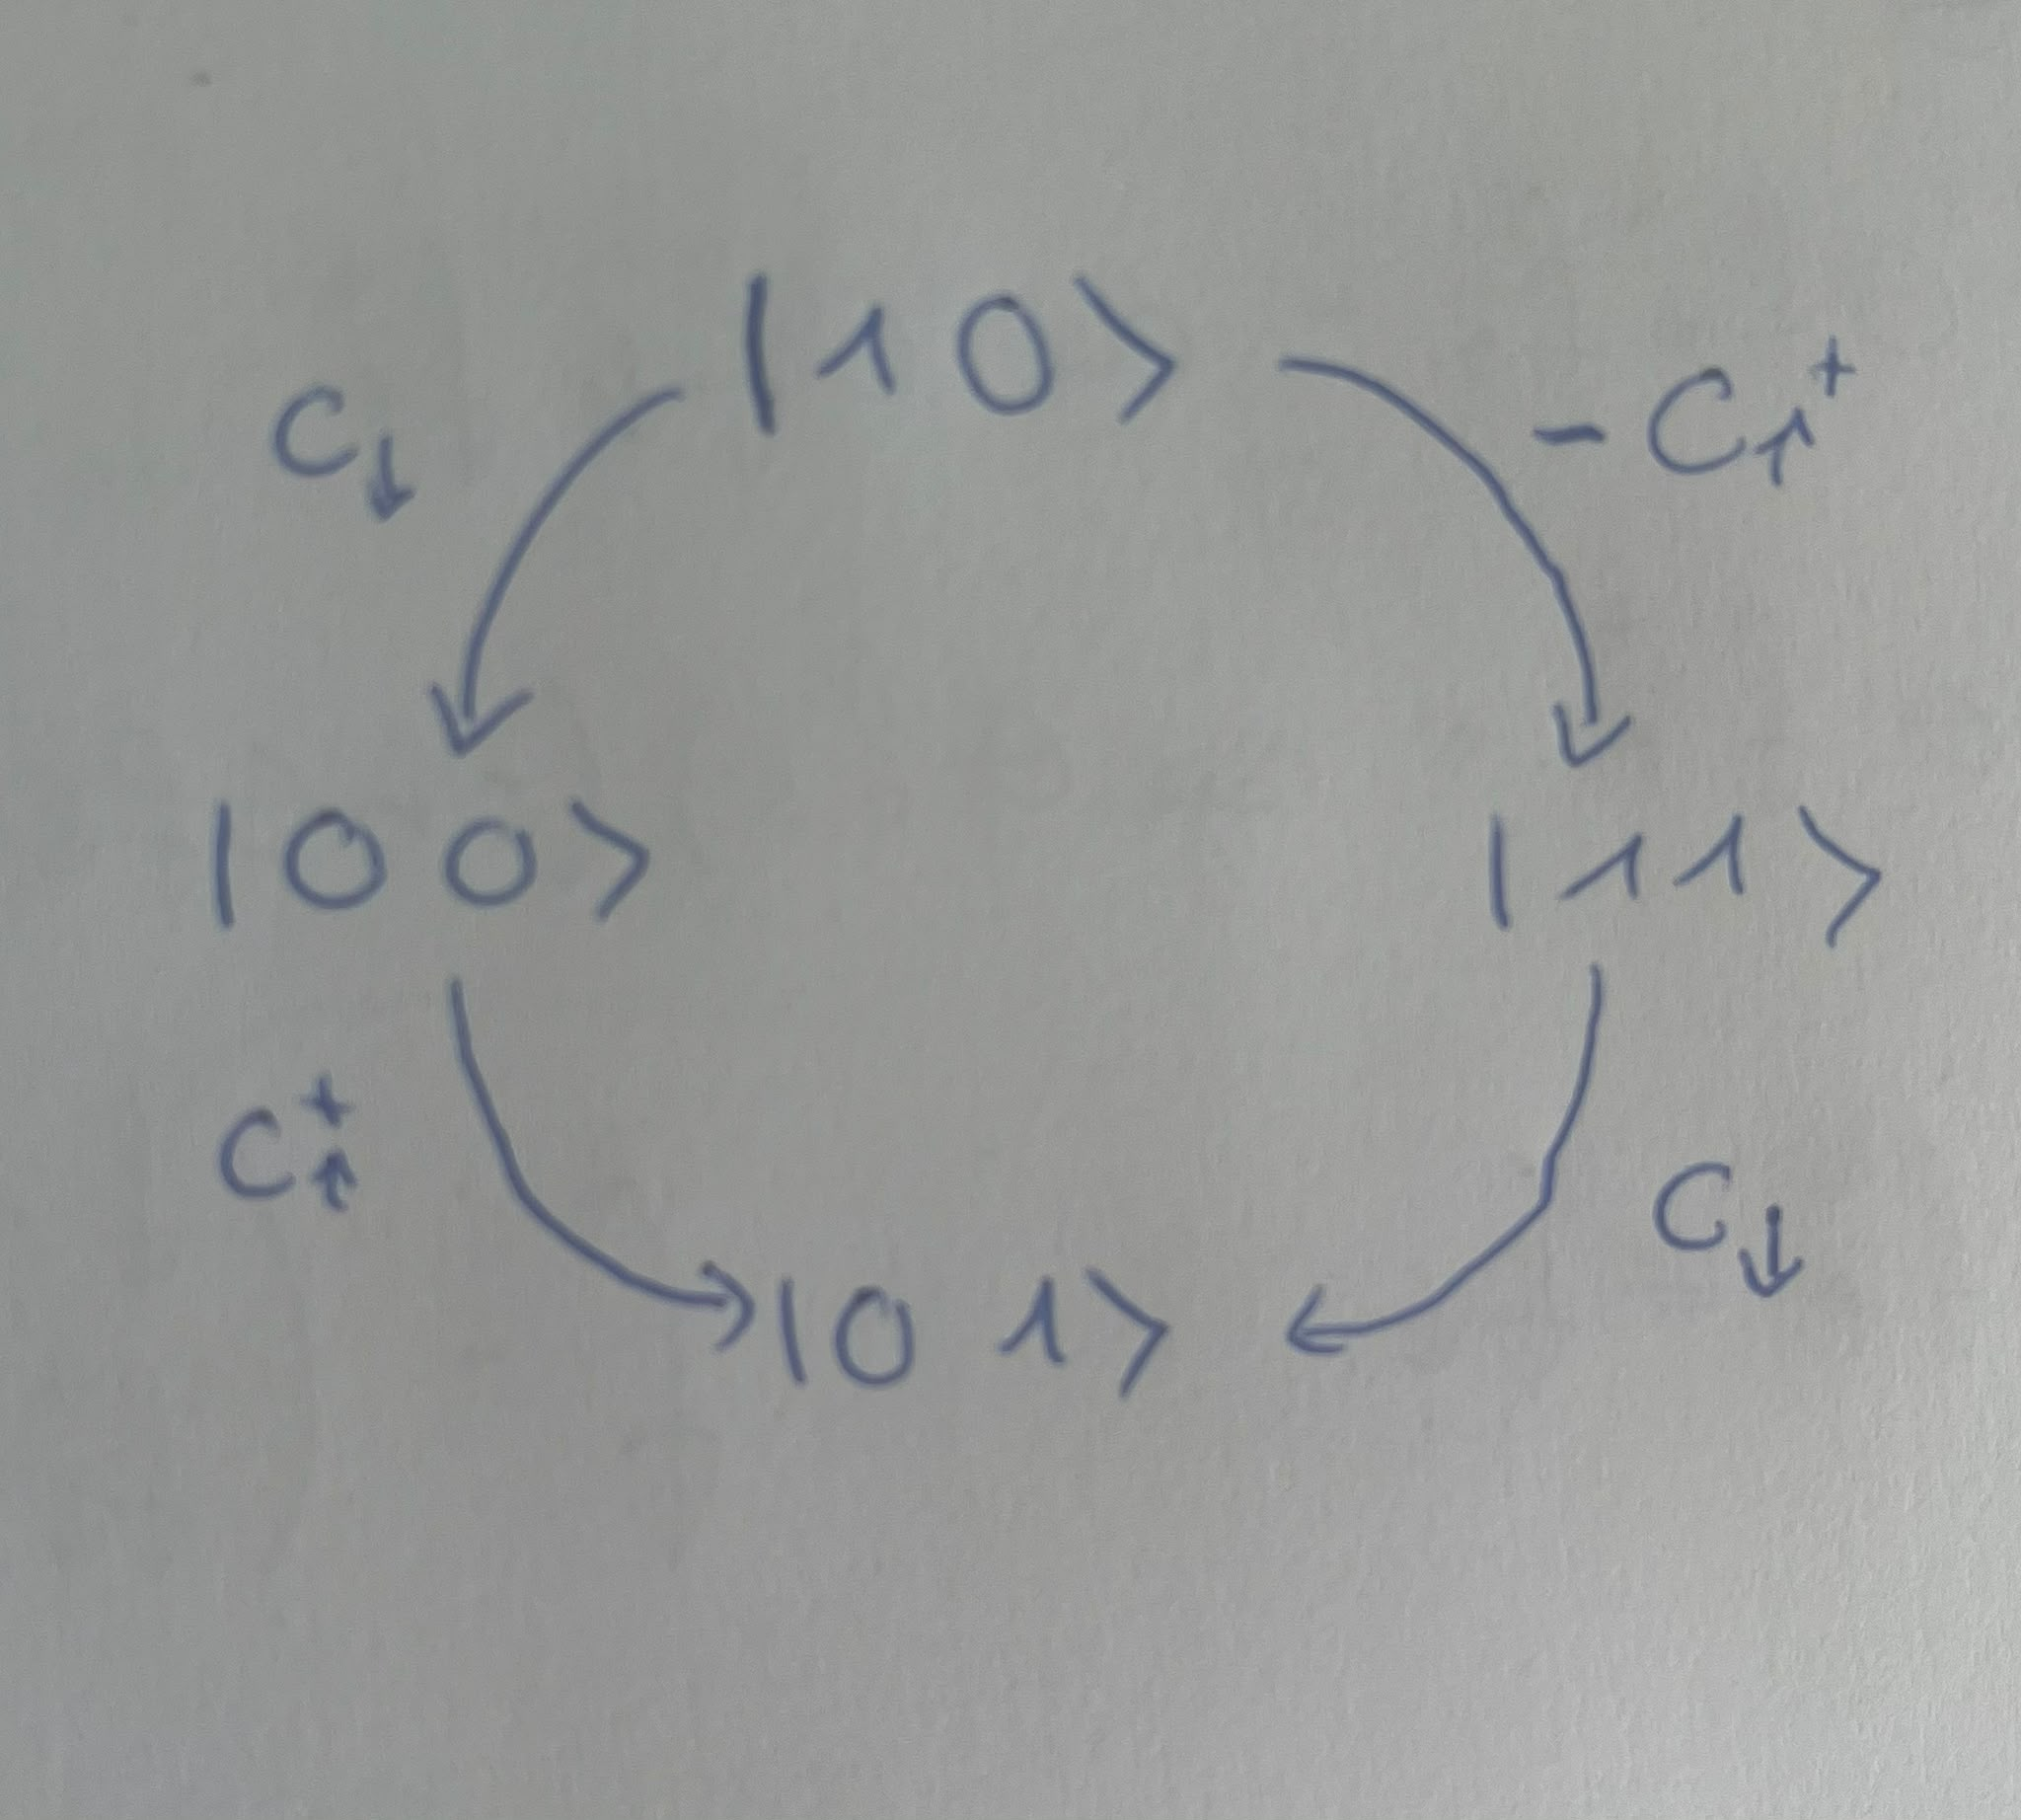
\includegraphics[width = 0.35\textwidth]{raising_operation.jpeg}.
\end{center}

Suddenly, we have a gauge-structure at our hands. The next questions come naturally: what are gauge transformations and what are gauge invariants? Staying with the example at hand:

\begin{equation}
\sin^2(\theta) c_\uparrow^\dagger c_\downarrow - \cos^2(\theta)c_\downarrow c_\uparrow^\dagger = 
\end{equation}








\end{document}
